	\documentclass[11pt]{article}
\usepackage[UTF8]{ctex}
\usepackage{picinpar,graphicx,bm}
\usepackage{booktabs}
\usepackage{diagbox}
\usepackage{float}
\usepackage{setspace}
\newcommand{\upcite}[1]{\textsuperscript{\textsuperscript{\cite{#1}}}}

% used to demo bracket for array
\usepackage{amsmath}

\usepackage{listings}
\usepackage{xcolor}
% 定义可能使用到的颜色
\definecolor{CPPLight}  {HTML} {686868}
\definecolor{CPPSteel}  {HTML} {888888}
\definecolor{CPPDark}   {HTML} {262626}
\definecolor{CPPBlue}   {HTML} {4172A3}
\definecolor{CPPGreen}  {HTML} {487818}
\definecolor{CPPBrown}  {HTML} {A07040}
\definecolor{CPPRed}    {HTML} {AD4D3A}
\definecolor{CPPViolet} {HTML} {7040A0}
\definecolor{CPPGray}  {HTML} {B8B8B8}
\lstset{
    columns=fixed,    
   % numbers=left,                                        % 在左侧显示行号
    frame=none,                                          % 不显示背景边框
    backgroundcolor=\color[RGB]{245,245,244},            % 设定背景颜色
    keywordstyle=\color[RGB]{40,40,255},                 % 设定关键字颜色
    numberstyle=\footnotesize\color{darkgray},           % 设定行号格式
    commentstyle=\it\color[RGB]{0,96,96},                % 设置代码注释的格式
    stringstyle=\rmfamily\slshape\color[RGB]{128,0,0},   % 设置字符串格式
    showstringspaces=false,                              % 不显示字符串中的空格
    language=c++,                                        % 设置语言
    morekeywords={alignas,continute,friend,register,true,alignof,decltype,goto,
    reinterpret_cast,try,asm,defult,if,return,typedef,auto,delete,inline,short,
    typeid,bool,do,int,signed,typename,break,double,long,sizeof,union,case,
    dynamic_cast,mutable,static,unsigned,catch,else,namespace,static_assert,using,
    char,enum,new,static_cast,virtual,char16_t,char32_t,explict,noexcept,struct,
    void,export,nullptr,switch,volatile,class,extern,operator,template,wchar_t,
    const,false,private,this,while,constexpr,float,protected,thread_local,
    const_cast,for,public,throw,std,size_t,__global__,__device__,__host__},
    emph={map,set,multimap,multiset,unordered_map,unordered_set,
    unordered_multiset,unordered_multimap,vector,string,list,deque,
    array,stack,forwared_list,iostream,memory,shared_ptr,unique_ptr,
    random,bitset,ostream,istream,cout,cin,endl,move,default_random_engine,
    uniform_int_distribution,iterator,algorithm,functional,bing,numeric,},
    emphstyle=\color{CPPViolet}, 
    frame=shadowbox,
    basicstyle=\footnotesize\ttfamily,
    tabsize=4,
}
\newcommand{\tabincell}[2]{\begin{tabular}{@{}#1@{}}#2\end{tabular}}


%layout
\usepackage{calc} 
\setlength\textwidth{7in} 
\setlength\textheight{9in} 
\setlength\oddsidemargin{(\paperwidth-\textwidth)/2 - 1in}
\setlength\topmargin{(\paperheight-\textheight -\headheight-\headsep-\footskip)/2 - 1.5in}


\title{《应用几何造型》读书报告  \begin{large} \hspace{1pt}----- \hspace{1pt}  曲面造型技术的调研\end{large} }
\author{11821095 葛林林}
\begin{document}
\maketitle
\section{引言}
曲面造型技术是图形学和应用几何造型领域较为活跃的核心问题之一,在计算机辅助设计、三维重建等课题有着极为广泛的应用。1963年Ferguson首先提出了将曲线曲面表示为参数的矢函数方法,这种利用参数形式对曲线曲面进行表示的方法后来成为工业界的标准。1964年至1967年麻省理工的Coons提出了具有一般性的曲面描述方法。1971年Bezier提出了利用伯恩斯坦基函数定义的Bezier曲线,该曲线可以控制曲线曲面的形状。70年代中期W.Gordon等人将B样条的理论应用到曲面的表示。随着发展曲面造型技术也日趋完善,然而该领域依然存在着许多急需解决的问题。
\par 本读书报告围绕曲面的表示方法和曲面造型技术的研究热点两个方面进行展开讨论,阐述了曲面造型技术中各种表示方法的基本概念、发展历程、各自的优缺点以及其应用领域,以及介绍了曲面造型领域一些研究热点和涉及的技术。

\section{曲面表示方法的介绍}
\subsection{参数曲面表示}
参数曲面是流形表示中最重要的一大类,参数曲面拥有易于绘制的优点,然而这种方法需要相对应的数据结构来表现连通性以及提高在图形渲染、碰撞检测等应用中的灵活性。除此之外,参数曲面不是直接的表示对象的内部或者外部使得很难进行bool操作。
\subsubsection{线框表示} 其优点是表示简单,缺点是表示的时候存在歧义。
\subsubsection{多边形表示}多边形表示法由顶点、边和面组成,能够有效的解决线框表示法存在的歧义问题。多边形表示法被广泛用于工业设计的模型存储当中,例如$ply$、$obj$文件格式都是基于多边形表示法。如下图所示是线框表示法的示意图。

\subsubsection{Bezier表示}
\paragraph{概念介绍} \mbox{}
\par Bezier曲面函数定义在Berstein基函数的基础上,可以利用控制顶点对曲面的形状进行控制。

\paragraph{历史发展} \mbox{}
\begin{table}[H]
\begin{tabular}{lp{16cm}}
1971年&法国Renault汽车公司的Bezier首次提出Bezier曲线的表示方法\upcite{survey1}。\\
\end{tabular}
\end{table}

\paragraph{优缺点} \mbox{}
\begin{table}[H]
\begin{center}
\begin{tabular}{ll}
\hline
\bm{优点}&\tabincell{l}{(1)只需要很少的点来表示曲面;\\(2)很容易控制形状。}\\
\hline
\bm{缺点}&\tabincell{l}{(1)Bernstein基是全局的;\\(2)次数是固定的(等于控制控制点的个数);\\(3)为了提高灵活性需要很高的次数;\\(4)很难保证光滑性;\\(5)很难与线求交;\\(6)很难与透射投影算法进行结合。}
\\
\hline
\end{tabular}
\end{center}
\end{table}

\subsubsection{B-spline表示}
它建立在B-spline基函数的基础上,通过控制顶点和阶次来控制曲面的形状。

\paragraph{历史发展} \mbox{}
\begin{table}[H]
\begin{tabular}{lp{16cm}}
1940s&该方法由Isaac Jacob Schoenberg首次提出\upcite{survey1}。\\
\end{tabular}
\end{table}

\paragraph{优缺点} \mbox{}
\begin{table}[H]
\begin{center}
\begin{tabular}{ll}
\hline
\bm{优点}&\tabincell{l}{(1)构造的曲面$C^0,C^1$连续\upcite{b-spline0}}\\
\hline
\bm{缺点}&\tabincell{l}{}
\\
\hline
\end{tabular}
\end{center}
\end{table}

\subsubsection{NURBS表示}


\subsection{细分曲面} 
\paragraph{概念介绍} \mbox{}
\par 细分曲面是通过从一个指定的粗糙的分段多边形网格出发,通过递归不断的将每个多边形切分成更小的面片从而逼近一个光滑的曲面。
\paragraph{发展历程} \mbox{}
\begin{table}[H]
\begin{tabular}{lp{16cm}}
1978年&由Edwin Catmull 和Jim Clark首次提出,随后Catmull和Clark\upcite{subdivision1},Doo和Sabin\upcite{subdivision2},Loop\upcite{subdivision3}分别进行了细化。\\
1994年& Hoppe等人\upcite{subdivision_ex1}将细分曲面应用到sharp feature的处理上。\\
1998年&DeRose等人\upcite{subdivision_ex2}在细分曲面上提出了subdivision mask的概念,并在此基础上提出了细分曲面的标量场。\\
2001年 & Displaced Subdivision Surface\upcite{DSS}由Aaron Lee、Henry Moreton和Hugues Hoppe在2001年的siggraph会议上提出,它便于几何压缩、编辑、动画制作,并且在图形渲染方面拥有很好的可扩展性和自适应性。\\
\end{tabular}
\end{table}

\paragraph{优缺点} \mbox{}
\begin{table}[H]
\begin{center}
\begin{tabular}{lc}
\hline
\bm{优点}&它不需要控制点的约束而能够表示任意拓扑类型。\\
\hline
\bm{缺点}&\tabincell{l}{(1)与参数曲面类似,它依赖于大量的数据结构\upcite{DF2};\\(2)需要处理特殊点\upcite{DF2};\\(3)难于控制和编辑\upcite{DF2}。}
\\
\hline
\end{tabular}
\end{center}
\end{table}

\paragraph{应用领域} \mbox{}
\par 细分曲面经常被用于三维动画角色的原型设计,如下图所示是《Geri's Game》中利用细分曲面得到的人物模型。


\subsection{隐式曲面表示} 

\paragraph{优缺点} \mbox{}
\begin{table}[H]
\begin{center}
\begin{tabular}{ll}
\hline
\bm{优点}&\tabincell{l}{(1)易于区分物体的内部和外部;\\(2)易于对象之间的混合。}\\
\hline
\bm{缺点}&\tabincell{l}{(1)进行求交运算非常耗时;\\(2)对于任意的物体很难找到对应隐式曲面。}
\\
\hline
\end{tabular}
\end{center}
\end{table}

\subsection{小波表示}
\subsection{距离场表示} 
\paragraph{概念介绍} \mbox{}
\par 距离场是一种离指定形状距离最近的标量场,该场用正负号来区分处于指定形状的内部或者外部\upcite{DF2}。
\begin{figure}[H]
\begin{center}
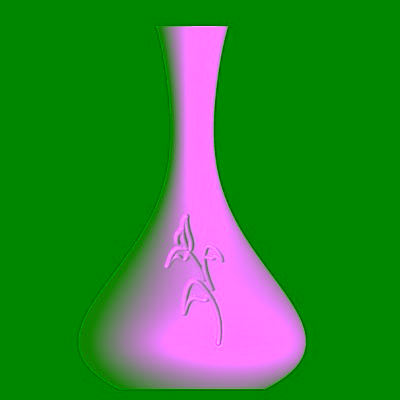
\includegraphics[scale=0.6]{DF.png}
\caption{距离场法表示的曲面(能够表示精细的曲面)}
\end{center}
\end{figure}

\paragraph{发展历程} \mbox{}
\begin{table}[H]
\begin{tabular}{ll}
1992年& Bradley A.Payne等人提出利用距离场的方法对曲面进行操作\upcite{DF1};\\
2000年&Sarah F. Frisken等人提出了ADFs算法\upcite{DF2},已解决距离场对于光滑和不光滑部分采样的不合理性导致的占用空间过大问题。然而该种方法没有从根本上解决曲面在离散表示时的细节损失问题\upcite{DF3}。\\
2001年&Jian Huang等人提出了一种完备的距离场表示法\upcite{DF3},在该文中作者指出了高质量的距离场需要满足的要求是准确、易于存储和传输。
\end{tabular}
\end{table}

\paragraph{优缺点} \mbox{}
\begin{table}[H]
\begin{center}
\begin{tabular}{ll}
\hline
\bm{优点}&\tabincell{l}{(1)能够很好的显示表面的细节;\\(2)能够很好的重建出曲面的位置和梯度。}\\
\hline
\bm{缺点}&\tabincell{l}{(1)常规采样情况下,为了很好的表示细节需要巨大的存储空间。}
\\
\hline
\end{tabular}
\end{center}
\end{table}

\paragraph{应用领域} \mbox{}
(1)碰撞检测;
(2)色域表示;
(3)计算机辅助加工。
\subsection{Normal Meshes}


\subsection{Semi-regular Meshes}

\subsection{Surfels}

\subsection{Wavelets}

\subsection{Adaptive Sampled Distance Fields}


\subsection{Multi-resolution Triangulation}


\section{研究热点}
\subsection{Sharp Feature的处理}

\subsection{High Density曲面处理}


\begin{thebibliography}{1}
\bibitem{b-spline0} Knott, Gary D. Interpolating cubic splines. Vol. 18. Springer Science \& Business Media, 2012.

\bibitem{subdivision1}Catmull, Edwin, and James Clark. "Recursively generated B-spline surfaces on arbitrary topological meshes." Computer-aided design 10.6 (1978): 350-355.

\bibitem{subdivision2} Doo, Daniel, and Malcolm Sabin. "Behaviour of recursive division surfaces near extraordinary points." Computer-Aided Design 10.6 (1978): 356-360.

\bibitem{subdivision3} Loop, Charles. "Smooth subdivision surfaces based on triangles." Master's thesis, University of Utah, Department of Mathematics (1987).

\bibitem{subdivision_ex1} Hoppe, Hugues, et al. "Piecewise smooth surface reconstruction." Proceedings of the 21st annual conference on Computer graphics and interactive techniques. ACM, 1994.

\bibitem{subdivision_ex2} DeRose, Tony, Michael Kass, and Tien Truong. "Subdivision surfaces in character animation." Proceedings of the 25th annual conference on Computer graphics and interactive techniques. ACM, 1998.

\bibitem{DSS} Lee, Aaron, Henry Moreton, and Hugues Hoppe. "Displaced subdivision surfaces." Proceedings of the 27th annual conference on Computer graphics and interactive techniques. ACM Press/Addison-Wesley Publishing Co., 2000.

\bibitem{normal-meshes} Guskov, Igor, et al. "Normal meshes." Proceedings of the 27th annual conference on Computer graphics and interactive techniques. ACM Press/Addison-Wesley Publishing Co., 2000.

\bibitem{surface-splatting}Zwicker, Matthias, et al. "Surface splatting." Proceedings of the 28th annual conference on Computer graphics and interactive techniques. ACM, 2001.

\bibitem{} Pauly, Mark, and Markus Gross. "Spectral processing of point-sampled geometry." Proceedings of the 28th annual conference on Computer graphics and interactive techniques. ACM, 2001.

\bibitem{DF1} Payne, Bradley A., and Arthur W. Toga. "Distance field manipulation of surface models." IEEE Computer graphics and applications 1 (1992): 65-71.

\bibitem{DF2} Frisken, Sarah F., et al. "Adaptively sampled distance fields: A general representation of shape for computer graphics." Proceedings of the 27th annual conference on Computer graphics and interactive techniques. ACM Press/Addison-Wesley Publishing Co., 2000.

\bibitem{DF3} Huang, Jian, et al. "A complete distance field representation." Proceedings of the conference on Visualization'01. IEEE Computer Society, 2001.

\bibitem{survey1} 刘壮, and 张乐年. "曲面造型技术综述." 智能制造 6(1997):20-22.
\end{thebibliography}



\end{document}